%%
%% This is file `mcmthesis-demo.tex',
%% generated with the docstrip utility.
%%
%% The original source files were:
%%
%% mcmthesis.dtx  (with options: `demo')
%% 
%% -----------------------------------
%% 
%% This is a generated file.
%% 
%% Copyright (C)
%%     2010 -- 2015 by Zhaoli Wang
%%     2014 -- 2016 by Liam Huang
%% 
%% This work may be distributed and/or modified under the
%% conditions of the LaTeX Project Public License, either version 1.3
%% of this license or (at your option) any later version.
%% The latest version of this license is in
%%   http://www.latex-project.org/lppl.txt
%% and version 1.3 or later is part of all distributions of LaTeX
%% version 2005/12/01 or later.
%% 
%% This work has the LPPL maintenance status `maintained'.
%% 
%% The Current Maintainer of this work is Liam Huang.
%% 
\documentclass{mcmthesis}
\mcmsetup{CTeX = false,   % 使用 CTeX 套装时,设置为 true
        tcn = 1902081, problem = C,
        sheet = true, titleinsheet = true, keywordsinsheet = true,
        titlepage = false, abstract = true}
\usepackage{palatino}
\usepackage{lipsum}
\usepackage{indentfirst}
\usepackage{booktabs}
\usepackage{graphicx}
\usepackage{enumitem}
\usepackage[section]{placeins} % 禁止图表跨过section
\setlength{\parindent}{2em}
\title{Drug Plague}
\author{\small \href{http://www.latexstudio.net/}
  {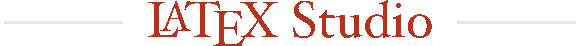
\includegraphics[width=7cm]{mcmthesis-logo}}}
\date{\today}
\begin{document}
\begin{abstract}


By performing data analysis, we determine several goals and construct corresponding models to reflect the hidden characteristics of the spread of the opioid crisis.\par

First, we conduct a series of data preprocessing work, including abnormal value processing, default value processing and data normalization. We then reclassify all the socio-economic factors included into 4 categories to analyze the data more efficiently. In order to consider the spread between adjacent counties, we also sort the data based on geographic location and adjacent relations.\par

Next, through the application of multiple linear regression model, we estimate the coefficients of various kinds of socio-economic factors, which reflect the relationship between elements and the number of drug reports. We discover that 38 factors have the most significant influence among all the possibilities. By comparing these coefficients, we find out the top 8 factors with the greatest effects on the condition of drug abuse.\par

Then, we introduce the index, comprehensive socio-economic property(CSE), to reflect the propensity for people in a county to use synthetic opioid or heroin. Based on the hierarchical cluster analysis(HCA), we firstly reduce the number of variables along with the consideration of common consensus. The HCA is a comprehensive index integrate multiple aspects, including family condition, education level and cultural background. Ranking CSE, we find that  the opioid crisis in Ohio is the most severe among the five states.\par

Finally, we revise the traditional Cellular Automata Model to simulate the spread of opioid crisis among counties. In our CA model, we shed the constraint by using arrays to store the neighbors, which implies that we can have theoretically infinite neighbors. We represent a county by a cell, and any two cells are adjacent in our CA model if and only if the two counties they respectively represent are geographically adjacent. Rules applied in our CA model, including prediction rules and backstepping rules, are devised to either forecast the trend in the future or estimate the situation in the past. The simulation of our CA model shows that Allegheny(PA), Hamilton(OH) and Philadelphia(PA) may be the places where the opioid crisis first started, while Delaware(PA) and Philadelphia(PA) might face a severe opioid crisis in the future. 
\begin{keywords}
Opioid Crisis; Drug Abuse; Socio-economic Factors 
\end{keywords}
\end{abstract}
\maketitle

\tableofcontents

\newpage

\section{Introduction}
\subsection{Problem Restatement}
As we all know, "drug" has never been a welcome word, which not only strongly endangers people's physical and mental health, but also seriously threatens social stability. Once people are exposed to drugs, they will develop strong dependence. After long-term use, they will be more delirious, impulsive, irritable and violent, which will lead to greater medical pressure, rising unemployment, rising crime rate and other negative social effects. Today, the so-called "drug" is not limited to traditional drugs such as heroin, but also includes the abuse of prescription sedatives, which has become a potential crisis in American society. Because opioids still play such a large role in medicine, it is not easy to achieve complete control.\par
To improve the effectiveness and ability of drug control, it is necessary to have a clear understanding of the mode of drug transmission. Generally speaking, drugs are mainly transmitted in the following three ways: first, through public entertainment places such as bars; second, through introduction among friends and relatives; third, through improper use of opioids in medical facilities. Due to the diversity of transmission modes, the concealment of drug taking process and the addiction of drugs themselves, drugs spread rapidly and covertly just like malaria. For the government, in addition to the huge difficulty in control, drug rehabilitation, treatment and reemployment for drug addicts are also worrying problems. In this regard, we will simulate the transmission mechanism of drugs and explore the source of drugs by tracing the source, so as to provide new ideas for drug control.\par

\subsection{Our Thinking}
We believe that the number of drug users in a region is closely related to some socio-economic factors. From a micro perspective, a person's choice to take drugs mainly depends on the prevalence of drugs around him and his own acceptance of drugs. The higher the prevalence, the greater the exposure to the drug for the individual, and thus the larger the population of drug users. However, an individual's acceptance of drugs is determined by his family background, education level, economic level and other social factors. Therefore, to understand the transmission characteristics of drug abuse behaviors, it is necessary to clarify the relationship between the number of drug users in a certain region and these socio-economic factors, so as to know which region is more prone to drug abuse.

\subsection{Our Goals}
\begin{figure}[!h]
\small
\centering
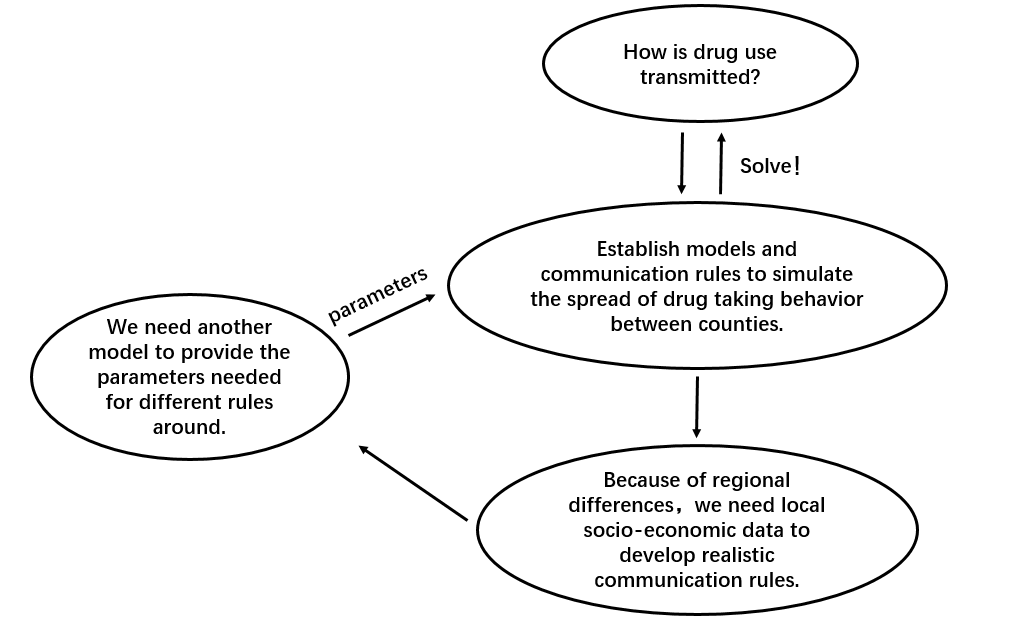
\includegraphics[width=12cm]{our_goal.png}
\caption{Flowchart for problem solving} \label{fig:our goal}
\end{figure}
Based on our understanding of the problem and the dataset provioded, we set the following goals:
\begin{enumerate}
\item Collate the big data of social economy and drug abuse reports of five states from 2012 to 2016.
\item Establish a model to describe the relationship between socio-economic factors and drug users in different five states, and find the factors that have the greatest influence on drug users.
\item Established a new model to simulate the spread of drug abuse behaviors in each county of the five states. We take the influence of adjacent counties into consideration. Use the social dataset from 2010 to 2016 to training to find the communication rules that best fit the actual situation.
\item Based on the rules in the existing model and the data in 2010, use the traceability analysis to find the most likely origin of initial drug transmission
\end{enumerate}

\section{Simplification and Assumptions}

Both the number of drug users and other socio-economic factors need to take into account the size and structure of the population. In reality, the movement and change of population are very complicated. To simplify the reality and take advantage of the value of the model, we make the following assumptions.\par
\begin{enumerate}
 \item  \textbf{The existence of drugs}\\
  Opioids will still be used due to medical needs. So laws and policies will not change in the short term.
 \item \textbf{Law enforcement stability}\\
  Regardless of the difference in police enforcement, The greater the number of drug users caught locally is, the greater the number of drug users locally is.
 \item \textbf{No externalities}\\
  Drug transmission within five states is affected only by five states and by interactions between them, not by other regions.
 \item \textbf{Communication equivalence}\\
  Any neighboring county has an equivalent degree of contact.
\end{enumerate}

\section{Data Preprocessing}
We get a set of rich detailed sampling investigation report on social and economic situation, including the locals of family, marriage situation, service level, language, place of birth, nationality, etc. of Kentucky, Ohio, Virginia, West Virginia and Pennsylvania this five states a total of 461 counties from 2010 to 2016. A total of 149 aspects. There is also data from a group of drug reports from the NFLIS in each of the five states, totaling more than 20,000. Due to the huge amount of data, there is the possibility of data missing and distortion in the original data, which will have a great impact on the prediction results of the model. So we need to preprocess the data.\par

\subsection{Default Value Processing}
We classified the missing data into the following two types:
\begin{enumerate}[label=\Alph*.]
\item \textbf{Multi-year data loss} \\
 We delete such data directly, because the data estimated with a small amount of data has no validity and cannot be used for our model.
\item \textbf{A small amount of data is missing}\\
 Some data are available for one or two years. Such data we use function interpolation method to improve the data set.
\end{enumerate}

\subsection{Abnormal Value Processing}
We think that abnormal data will also affect the prediction and simulation of the model. In the socio-economic report data set of five states, the confidence interval of this set of data is given based on margin of error. If the expected value is within the confidence interval, the data is accepted; otherwise, the data is rejected.


\subsection{Normalization of Data}
The data set structure of socio-economic category is complex, and the data values vary greatly due to the differences in practical significance. In order to accurately represent the influence of socio-economic factors on the spread of drug abuse behaviors, the data need to be normalized. We use the max-min method (\ref{equ:X equation})to transform the original data into a dimensionless expression that becomes a scalar. 
  %$$ X_{norm} = \frac{X- X_{min}}{X_{max}-X_{min}} \eqno{(1)}$$
  \begin{equation}  \label{equ:X equation}
X_{norm} = \frac{X- X_{min}}{X_{max}-X_{min}}  
  \end{equation}


\subsection{Reclassification and Integration of Social Data}
The original data has been preliminarily classified. For example, the economic and social data has been divided into 17 categories (16 categories from 2010 to 2012, lacking the category of Internet use). Not all the categories are the data required by the model. At the same time, some data are classified too trivial, which is not conducive to the simplification of the model. Therefore, we re-screen and classify these 17 categories, forming four categories in total:

\begin{enumerate}[label=\Alph*.]
\item \textbf{Family background}\\
 Is the data about the number of different types of families in local statistics, including household, relation, children, marriage and etc.
\item \textbf{Education level}\\
 Data describing local educational resources and educational level of residents. Including the number of primary and secondary schools, local residents have educational level.
\item \textbf{Proportion of specific population}\\
 It describes the proportion of a specific population in the local area, including the number of veteran and the number of disabled people.
\item \textbf{Cultural background}\\
 Data describing the overall cultural composition and cultural environment of local residents, including place of birth, place of residence one year ago, level of language use, time spent living there and ancestors.
\end{enumerate}

\subsection{Relationship of Adjacence} 
We want to characterize the spread of drug use across 461 counties in five states, so we need the geographic location and proximity of the counties. To get this data, we processed the map and labeled each county. For each county, all the Numbers of its neighboring counties are stored as an array, forming a map of 461 counties. \par

\subsection{Proportion of substances in Drug Reports} 
Fig.\ref{fig:proportion of drug reports} shows the proportion of different substances in drug reports.

\begin{figure}[!h]
\small
\centering
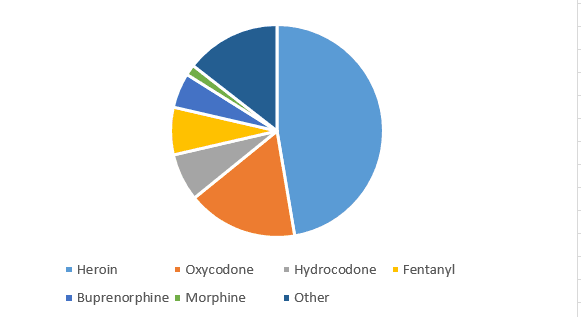
\includegraphics[width=8cm]{proportion.png}
\caption{Proportion of substances in Drug Reports} \label{fig:proportion of drug reports}
\end{figure}



\section{The Multivariable Linear Regression Model(MLR)}

\subsection{Construction of MLR}

  We develop a multivariable linear regression model to analyze the differences between the number of drug reports among counties. According to the data provided from 2010 to 2016, we make an elementary assumption that there is a linear relationship between independent variables and the number of drug reports. Since there are many possible socio-economic factors relative to the results, the multivariable linear regression model can explain the complexity of the system and explore the most important factors that contribute to the results more comprehensively and accurately.\par

  \subsection{Symbols}


\begin{table}[!h]
\centering
\caption{Main Symbols used in MLR Model} %\label{tab:aStrangeTable}
\begin{tabular}{ll}
\toprule[2.5pt]
\textbf{Symbols}& \textbf{Definition} \\
\midrule[1.5pt]
 $l_k$   & the index of some county     \\
 \midrule
 $x_{l_k}^i$ & the data of HC01\_VC\_i of the county whose index is $l_k$   \\
 \midrule
 $p_{l_k}$ & the number of drug reports of the county whose index is $l_k$  \\

\bottomrule
\end{tabular}
\end{table}

  To reflect the hidden relationship between the severity of drug abuse and various factors, we include as many possible factors as we can to modify our multivariable linear regression model. \par

  Assume $\beta_i$ to be the regression coefficient of $x_i$. 

  We introduce a basic multivariable linear equation to the model:
    \begin{equation}
     \left\{ 
        \begin{array}{ll}
        &  \boldsymbol{P}  =  \beta_0 + \beta_1 \boldsymbol{x_1} + ... + \beta_n \boldsymbol{x_n} + \boldsymbol{\epsilon}  \\
        &  E(\boldsymbol{\epsilon})  =  0 \\
        & COV(\boldsymbol{\epsilon},\boldsymbol{\epsilon}) = \sigma ^2 I_n
        \end{array}
    \right. 
    \end{equation}
    where $\boldsymbol{P}=[p_{l_1},...,p_{l_n}]^{T}$, $n$ denotes the number of counties, $\boldsymbol{x_i}=[x_{l_1}^i,...,x_{l_n}^i]^{T}$,  $I_n$ is the identity matrix, $\sigma ^2$ is the variance of $\boldsymbol{\epsilon}$.

\subsection{Results}
  Since the system involves quite a lot of underlying factors and there is complex multiple linearity between several elements, we used stepwise regression to better calculate the data. 

      \begin{table}[!h]
      \centering
      \caption{Coefficients of some key factors} \label{tab:Coefficients}
      \begin{tabular}{lll}
      \toprule[2.5pt]
      \textbf{Code}& \textbf{Coefficient}  & \textbf{Meaning}\\
      \midrule[1.5pt]
      HC01\_VC11 & 3.0505 & HOUSEHOLDS BY TYPE - Family households(families)\\
      \midrule
      HC01\_VC144& 2.6515 & Population born outside the United States  \\
      \midrule
      HC01\_VC12& -2.6013 &  HOUSEHOLDS BY TYPE - Family households (families) - Female \\
      & &  householder, no husband present, family- With own children under 18  \\
      \midrule
      HC01\_VC151 & -2.5784 & YEAR OF ENTRY - Entered 2010 or later \\
      \midrule
      HC01\_VC28 & 1.572 & RELATIONSHIP - Child\\
      \midrule
      HC01\_VC14 & 1.3058 & HOUSEHOLD BY TYPE - Nonfamily households - Householder  \\
      \midrule 
      &  & living alone\\
      \midrule
      HC01\_VC177 & -1.2417 & LANGUAGE SPOKEN AT HOME - Language other than English - \\
      & & Other languages\\
      \midrule
      HC01\_VC91 & 1.0572 & EDUCATIONAL ATTAINMENT - Graduate or professional degree\\
      \bottomrule
      \end{tabular}
      \end{table}

      Table.\ref{tab:Coefficients} shows us a lot of information. ‘Family households(families)’, ‘Population born outside the United States’ have the greatest promoting influence on the number of drug reports. While ‘Family households (families) -Female householder -With own children under 18 years’ and ‘YEAR OF ENTRY - Entered 2010 or later’ restrain the acceleration of drug abuse.

\begin{figure}[!h]
\small
\centering
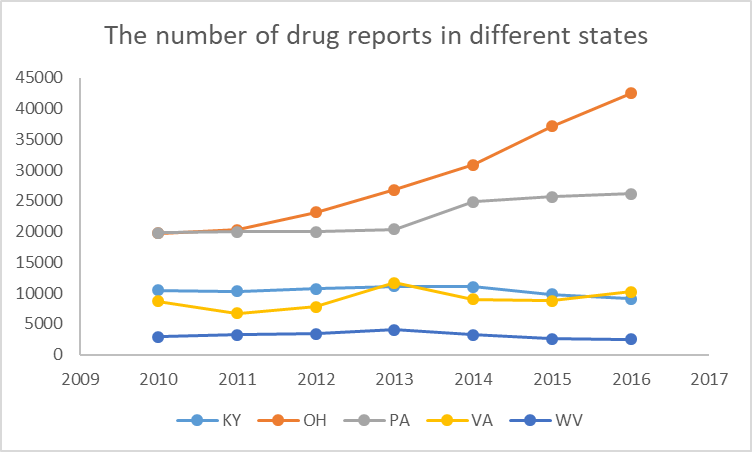
\includegraphics[width=8cm]{MLR_DRUG_REPORTS.png}
\caption{The number of drug reports in different states} %\label{fig:neighbors}
\end{figure}

\begin{figure}[!h]
\small
\centering
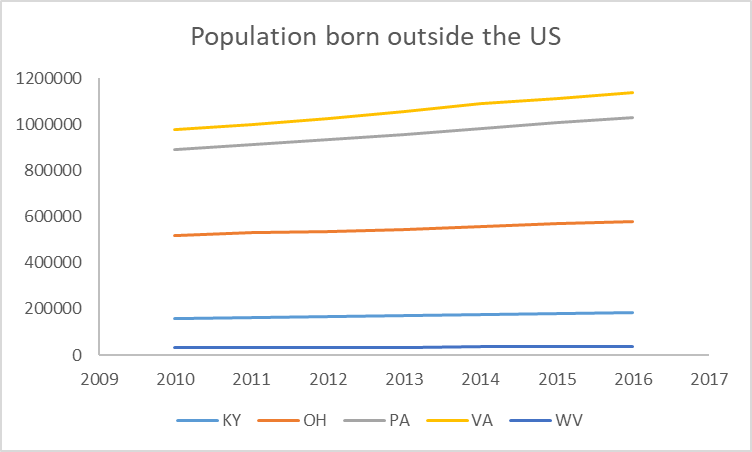
\includegraphics[width=8cm]{MLR_POPULATION.png}
\caption{Population born outside the US} %\label{fig:neighbors}
\end{figure}


\section{Comprehensive Evaluation System} 

In this part, we develop a evaluation system to introduce a specific characteristic of a county, which can efficiently reflects the local condition of synthetic opioid and heroin use. \par

\subsection{Hierarchical Cluster Analysis(HCA)}
Through the analysis above, we find 38 possible factors with the most significant influence. To analyze the data more efficiently and reduce the number of variables, we then categorize these factors based on cluster analysis along with common consensus. 
All the data involved have been normalized, therefore, we do not consider the difference between dimensions. When conducting hierarchical cluster analysis, we choose squared Euclidean distance as the metric to measure the dissimilarity between sets of observations. The formula is showed below:
    \begin{equation} || x^i - x^j||_2^2= \sum\limits_{k} (x_{l_k}^i - x_{l_k}^j)^2 \end{equation}
   The results of classification based on HCA is shown in Fig.\ref{fig:classification}. And the meaning of notations in Fig.\ref{fig:classification} can be found in Table.\ref{tab:some notations}
\begin{figure}[h]
\small
\centering
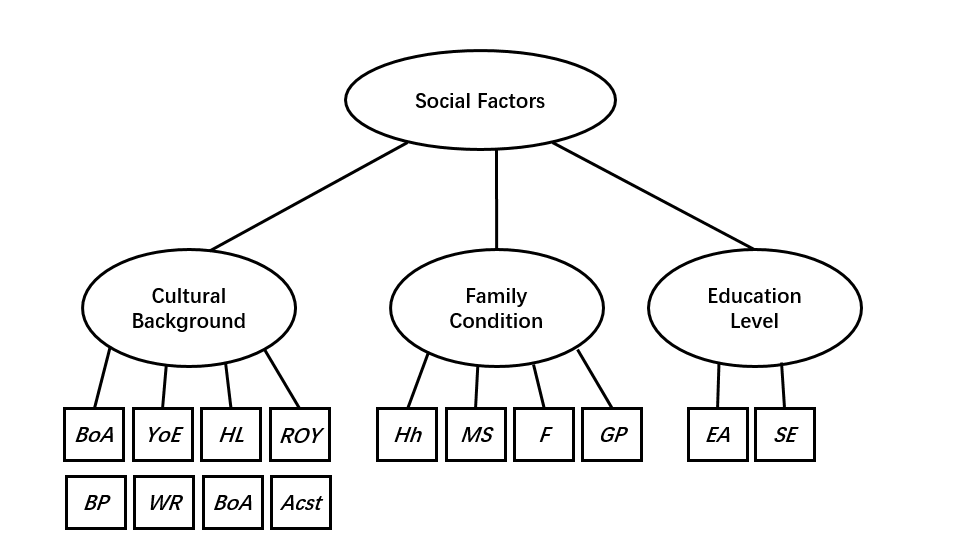
\includegraphics[width=8cm]{Classification.png}
\caption{Classification based on HCA} \label{fig:classification}
\end{figure}


\begin{table}[!h]
\centering
\caption{Some notations} \label{tab:some notations}
\begin{tabular}{ll}
\toprule[2.5pt]
\textbf{Notations}& \textbf{Meaning} \\
\midrule[1.5pt]
 BOA   & Population born outside the United States    \\
 \midrule
 YoA & Year of entry   \\
 \midrule
 HL & Language spoken at home  \\
  \midrule
 BP & Place of Birth \\
  \midrule
 ROY & Residence 1 year ago \\
  \midrule
 WR & World region of birth of foreign born \\
  \midrule
Acst & Ancestry \\
 \midrule
Hh & Households by type \\
 \midrule
MS & Marital status \\
 \midrule
GP & Grandparents \\
 \midrule
F & Fertility \\
 \midrule
EA & Educational attainment \\
 \midrule
SE & School enrollment\\
\bottomrule
\end{tabular}
\end{table}



\subsection{Construction of CSE} 
The core index of our evaluation system is called comprehensive socio-economic property(CSE), which reflect the propensity for people in a county to use synthetic opioid or heroin. The CSE consists of family condition(FAC), education level(EDL), cultural background(CUB), each of them including several indexes. \par


To evaluate the correlations between a county’s drug reports and its family condition, education level, cultural background, for every category, we represent the correlation by the mean of this category’s correlation coefficients $\beta_i$  respectively. If the mean is relatively larger, we consider the correlation between drug reports and the factors of this category to be significant. \par
We introduce a set of classifications as follows:
  $$ C = \{FAC,EDL,CUB\}$$
  where $FAC$ is an index set of factors included in family condition, $EDL$ is an index set of factors included in education level, $CUB$ is an index set of factors included in cultural background.
  We also introduce two definitions as below:

\begin{table}[!h]
\centering
\caption{Main Symbols used in CSE} %\label{tab:aStrangeTable}
\begin{tabular}{ll}
\toprule[2.5pt]
\textbf{Symbols}& \textbf{Definition} \\
\midrule[1.5pt]
 $T_{\alpha}$ & the index of elements included in set $\alpha$, where $\alpha \in C$\\
 \midrule
 $c_{\alpha}$ & the control coefficient of classification of $\alpha$ \\

\bottomrule
\end{tabular}
\end{table}
We can calculate $c_{\alpha}$ approximately by the following formula:
\begin{equation}  c_{\alpha} = \frac{\sum \beta_i}{|T_{\alpha}|}, i \in \alpha \end{equation}

On the other hand, we evaluate the specificity of some category by the variance of correlation of factors in this category. If the variance is small, the factors in this category are similar correlated to the number of drug reports. The formula to calculate the variance is as follows:
\begin{equation}   s_{\alpha} = \frac{\sum (\beta_i - \bar{\beta_{\alpha}})^2}{|T_{\alpha}|}, i \in \alpha  \end{equation}
where $\bar{\beta_{\alpha}} = \frac{\sum \beta_i}{\alpha}, i \in \alpha$

Based on above, we can introduce a parameter $\mu$ to reflect the propensity for people in a county to use synthetic opioid or heroin. In order to achieve this, we need to introduce two constants below:

\begin{table}[!h]
\centering

\begin{tabular}{ll}
\toprule[2.5pt]
\textbf{Symbols}& \textbf{Definition} \\
\midrule[1.5pt]
 $M_{\alpha}$ & the maximum of the average of all the data of factors \\
 \midrule
 $m_{\alpha}$ & the minimum of the average of all the data of factors \\

\bottomrule
\end{tabular}
\end{table}
We assume $x_{\alpha}$ to be a county's average data of factors in set $\alpha$.

Then we can calculate $\mu$ by the following formula:
\begin{equation} \mu = \sum c_{\alpha} \frac{x_{\alpha}-m_{\alpha}}{M_{\alpha}-m_{\alpha}} \end{equation}

We name $\mu$ as CSE index. The larger the $\mu$ of some county is, the more likely the residents in this county to be addicted to synthetic opioid or heroin.

\subsection{Results of Evaluation}

Through the curve fitting based on the data of counties in five states provided, we can obtain the estimate value of some parameters mentioned before.

\begin{table}[!h]
\centering
\begin{tabular}{l|lll}
\toprule
 & FAC& EDL & CUB\\
\midrule
  $M_{\alpha}$& 96652& 78253& 49200\\
  $m_{\alpha}$& 114& 78&49\\

\bottomrule
\end{tabular}
\end{table}

With these parameters and the formula we obtained before, we can evaluate the inclination of drug abuse in a county approximately. Through our assessment, we find some characteristics of the factors related to drug abuse. 
\begin{enumerate}[label=\alph*.]
\item \textbf{Family condition}\\ 
Among the three basic classifications, family condition has the greatest impact on the fluctuation of the number of drug reports. The addiction to synthetic opioid or heroin can be viewed as a kind of psychiatric disorder, while the significance of the family to build a healthy personality has long been recognized since Freud. Through the past two decades, including family as a special way to treat mental problems has gained much attention. 
\item  \textbf{Education}\\
  Education also plays an important role in the development of personality. According to a book written by Bachman and Jerald G, \emph{The education-drug use connection : how successes and failures in school relate to adolescent smoking, drinking, drug use, and delinquency}, people who is successful in school or obtain higher education also tend to enjoy a broad range of outcomes in their lives. The education a person received varies a lot and will exert much impact on one’s future.
\item  \textbf{Cultural background}\\
Through our model testing, we find that cultural background also relates closely to the number of drug abuse reports. Among all the factors involved in cultural background, the coefficient of ‘population born outside the United States’ reaches 2.65, while the coefficient of ‘the number of people who speak languages other than English’ is only -1.24. These show us that there is a great difference between people living in different backgrounds.
\end{enumerate}


\section{CA Model}

To consider the relationship between adjacent counties, CA Model is introduced. Due to the specificity of this problem, we will modify the traditional CA Model to satisfy the limitations of this problem. \par


\subsection{Properties} % or maybe description

CA Model is consisted of multiple cells with state and the relartionship of adjacence. Here we present several properties regarding our revised CA Model. 

\begin{itemize}
\item In our revised CA Model, a cell represents some county in the five states.
\item The state of a cell denotes the number of predicted drug reports of some county.
\item Any two cells are adjacent in CA Model if and only if the two counties they respectively represent are geographically adjacent.
\item In a new stage, some cell's state is determined by this cell's state and its neighbors' state in the previous stage.
\end{itemize}

Our revised CA Model differs from traditional CA Model in several aspects: 
\begin{enumerate}
\item \textbf{Number of  states}.\\
As the state of cell is equivalent to the number of some county's drug reports, the cell in our revised CA Model has infinite kinds of state. However, the cell in traditional CA Model are restricted to finite kinds of state.
\item \textbf{Number of neighbors}\\
Traditional CA model has to restrict the number of neighbors to be 4 or 8. In our CA Model, we shed the constraint by using arrays to store the neighbors, which implies that we can have theoretically infinite neighbors.
\end{enumerate}

\begin{figure}[h]
\small
\centering
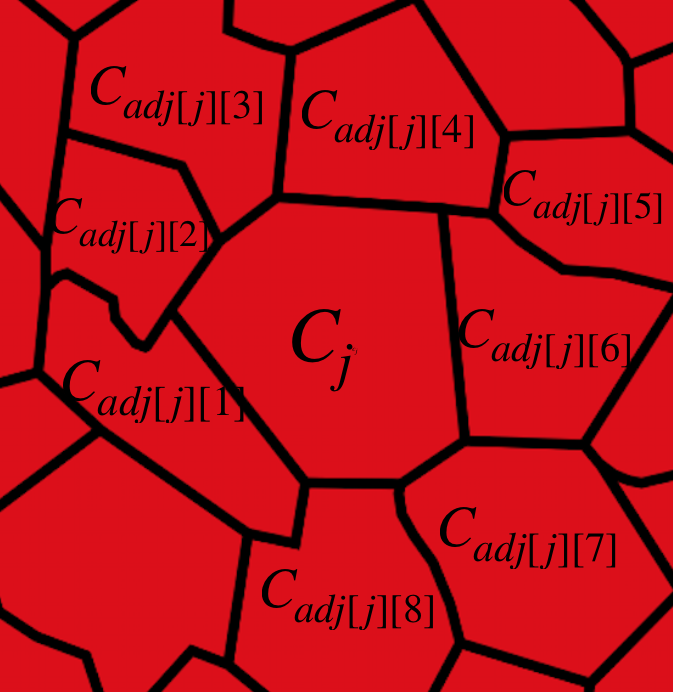
\includegraphics[width=8cm]{CA_rules.png}
\caption{neighbors} \label{fig:neighbors}
\end{figure}


\subsection{Symbols}


\begin{table}[!h]
\centering
\caption{Main Symbols used in CA Model} %\label{tab:aStrangeTable}
\begin{tabular}{ll}
\toprule[2.5pt]
\textbf{Symbols}& \textbf{Definition} \\
\midrule[1.5pt]
$c_j$ & the $j_{th}$ cell \\
\midrule
$s_{ij}$& the $j_{th}$ cell's state in stage $i$ \\
\midrule
$s_{ij}'$& the $j_{th}$ cell's state in stage $i$ (only for backstepping)\\
\midrule
$r_{ij}$ & the $j_{th}$ cell's real data in stage $i$ \\
\midrule
$n_{j}$ & the number of the $j_{th}$ cell's neighbors\\
\midrule
$adj[j]$ & the array which stores the $j_{th}$ cell's neighbors \\
 & We can use $adj[j][k]$ to index the neighbors of the cell, where $k = 1,...,n_{j}$\\
\midrule
$N$ & the number of counties in the five States\\
\midrule
$\lambda$ & a constant which describes the degree of adjecnt counties's contact \\
\bottomrule
\end{tabular}
\end{table}


\newpage
\subsection{Prediction Rules }
Any cell's state in the $(i+1)_{th}$ stage is determined by its state and its neighbors' state in the $i_{th}$ stage. In other words, $s_{(i+1)j}$ is determined by $s_{ij}$ and $s_{ik}$ where $c_k$ is a neighour of $c_j$.\par
With careful consideration, We choose the relationship to be linear. The Prediction formula is as follows.
      \begin{equation} s_{(i+1)j} \ = \ k_1 s_{ij} \ + \ k_2 \lambda \frac{\sum\limits_{k=1} ^{n_j} s_{i (adj[j][k])} }{n_j} \end{equation}
    where $k_1$ denotes the influence of its own state, $k_2$ denotes the infulence of its neighbors' state, $\lambda$ is a constant which describes the degree of adjecnt counties's contact. After multiple tests and the consideration of reality, we choose $\lambda$ to be 0.3.\par

    This Prediction formula takes both the cell's influence and its neighbors' influence into consideraion.
\subsection{Backstepping Rules}
    We also need to estimate the data in years before 2010 which is not provided. We simply rewrite the formulation above and make some approximation. To distinguish Prediction formula, we use $s_{ij}'$ to replace $s_{ij}$. The formula is as follows:

       \begin{equation} s_{ij}' = \frac{s_{(i+1)j}'}{k_1} - \frac{k_2}{k_1} \lambda \frac{\sum\limits_{k=1} ^{n_j} s_{(i+1) adj[j][k]}' }{n_j} \end{equation}
      
      where $k_1$ , $k_2$ and $\lambda$ are identical to those in Prediction Rules. 

\subsection{Determine Coefficients} \label{Section:Determine coefficients}
    To determine the coefficients $k_1$ and $k_2$, we use program to help us choose between $0$ and $1$ automatically. We have data about drug reports in years 2010-2017. The program will choose between $0$ and $1$ by step $0.001$  to minimize the error. The formula to calculate error is as follows.
    \begin{equation} error = \frac{\sum\limits_{i=2011}^{2017} \sum_{j=1}^{N} (r_{ij} - s_{ij})^2  }{N * (2017-2011+1)} \end{equation}
    where $N$ is the number of counties in the five state. \par
    Given $\lambda=0.3$, we find the error is minimal when $k_1=0.999$ and $k_2=0.186$. Based on this, we can conclude that the cell's own influence is of most significance, but the influence of adjacent cells cannot be ignored.

\subsection{Appliance of the CA Model}

\begin{figure}[!h]
\small
\centering
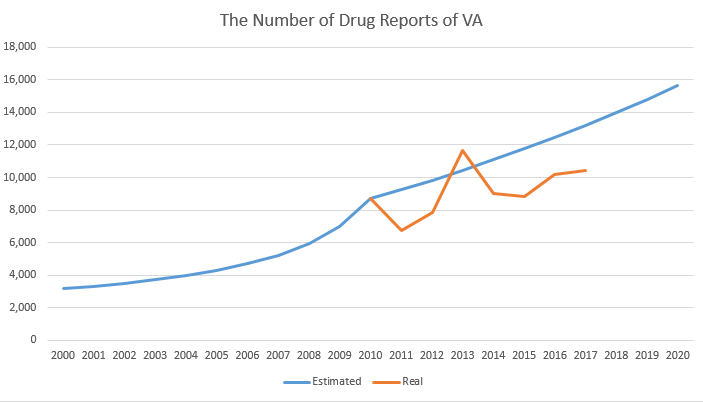
\includegraphics[width=9cm]{CA_of_VA.png}
\caption{The number of drug reports of VA} \label{fig:CA_of_VA}
\end{figure}

\begin{figure}[!h]
\small
\centering
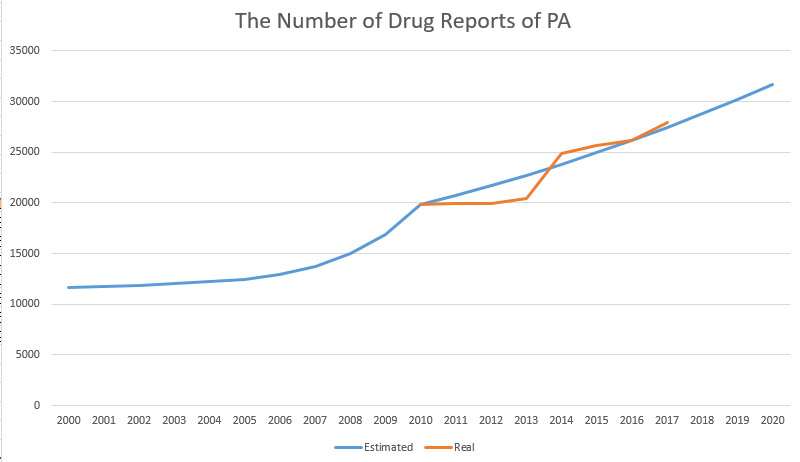
\includegraphics[width=9cm]{CA_of_PA.png}
\caption{The number of drug reports of PA} \label{fig:CA_of_PA}
\end{figure}

  We have estimated the number of drug reports of every county in years from 2000 to 2030 using our revised CA model. Therefore we can estimate the data of every state by summing the data of its counties. Fig.\ref{fig:CA_of_VA} shows the estimated data and real data of VA. And Fig.\ref{fig:CA_of_PA} shows the estimated data and real data of PA. CA Model fits well with the State PA, where two lines are very close. As to the State VA, two lines have similar trends.\par
  Using CA Model, we can get data of counties, which means we can get geographical distribution of data. This may provide insight into the data. 
\begin{figure}[!htbp]
\small
\centering
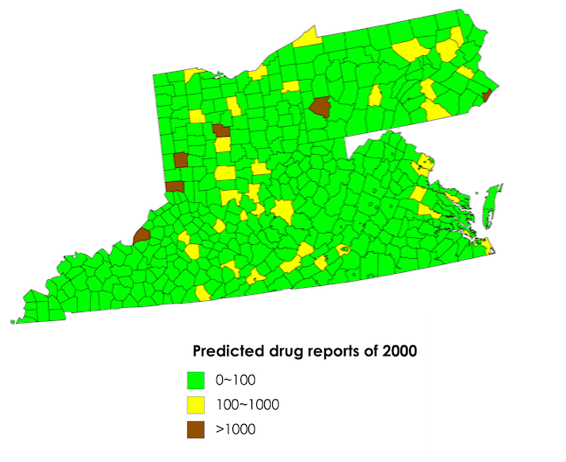
\includegraphics[width=10cm]{CA_2000.png}
\caption{Estimated Geographical Distribution in the year 2000} \label{fig:CA_2000}
\end{figure}

\begin{figure}[!htbp]
\small
\centering
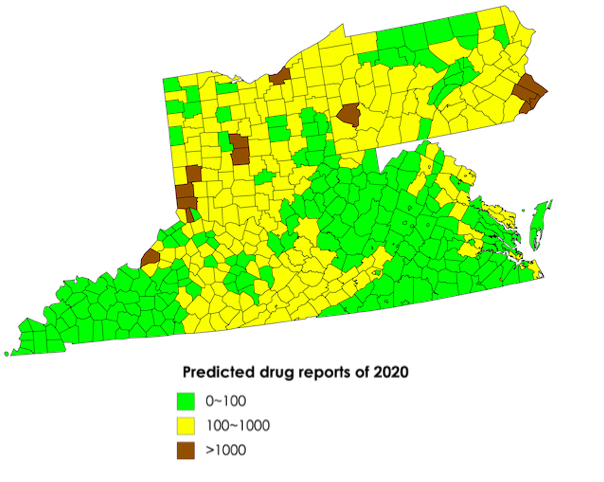
\includegraphics[width=10cm]{CA_2020.png}
\caption{Estimated Geographical Distribution in the year 2020} \label{fig:CA_2020}
\end{figure}

In Fig.\ref{fig:CA_2000}, there are six counties with estimated numbers greater than $1000$ in the year 2000, namely Delware(OH)  , Jefferson(KY), Montgomery(OH), Allegheny(PA), Hamilton(OH), Philadelphia(PA). In Fig.\ref{fig:CA_2020}, there are thirteen counties with estimated numbers greater than $1000$ in the year 2020. We can notice that the growth in number spread from the red regions in Fig.\ref{fig:CA_2000}. Therefore we may conclude that the drug abuse might have started form the red regions in Fig.\ref{fig:CA_2000}.


\subsection{Sensitivity Analysis}
  As the constant $\lambda$ in CA Model may be hard to obtain or there might be some uncertainty, the choice of $\lambda$ might affect the result of our CA Model. So in order to test the robustness of our revised CA Model , a sensitivity analysis is conducted by testing our CA Model with various $\lambda$. \par
  Here we calculate the error by the formula in Section \ref{Section:Determine coefficients}. We originally choose $\lambda=0.3$. To test the robustness of our CA Model, we set $\lambda=0.5$ and $0.8$ respectively. The tests (Table.\ref{tab:sensitivity analysis}) showed that our model is robust.

  \begin{table}[!h]
\centering
\caption{The influence of $\lambda$'s change on error}
 \label{tab:sensitivity analysis}
\begin{tabular}{ccc|c}
\toprule[2.5pt]
$\lambda$ & $k_1$ & $k_2$ & error \\
\midrule[1.5pt]
0.3 \ \ \ \ &  \ \ \ \ 0.999 \ \ \ \ & \ \ \ \ 0.186 \ \ \ \ & \ \ \ \ 78691.4 \\
\midrule
0.5 \ & \ 0.999 \ & \ 0.112 \ & \ 78694.1 \\
\midrule
0.8 \ & \ 0.999 \ & \ 0.070 \ & \ 78694.1 \\
\bottomrule
\end{tabular}
\end{table}

\section{Conclusion}
  To find out the significant factors of the underlying opioid crisis and the characteristics hidden in the spread, we build two models. Multiple Linear Regression Model(MLR) is constructed to find the correlations between different factors and the number of drug reports. Based on Cluster Analysis, we introduce CSE index to evaluate the propensity for people in a county to use synthetic opioid or heroin. We also revise the traditional Cellular Automata Model to simulate the spread of opioid abuse among counties. \par
 With the application of our models, we find some meaningful and profound insights: 
 \begin{enumerate} 
  \item The spread of opioid use might have started in the following locations: Allegheny(PA), Hamilton(OH) and Philadelphia(PA).
  \item If this spread continues, the situation may continue deteriorating. By the year of 2020, Delaware(PA) and Bucks(PA) will be listed in the most severe counties.
  \item The possible factors of the underlying opioid crisis are as follows:
    the population born outside the United States, the number of householders living alone and the number of children in households.
  \item Veterens, bachelors and divorcee are latent users of opioid.
 \end{enumerate}

\section{Strength and Weakness}

\subsection{Strength}

\begin{enumerate}
\item Universality. Our model showed a small deviation between the simulated situation and the actual situation in 2016 after iterating with data from five states in 2010 separately. Therefore, we believe that our model has a strong universal value. After obtaining the socio-economic data believed by a new region and the drug abuse report, our model can better simulate the spread of drug abuse behavior in the local area, so as to provide help for the local government in drug prevention and control.
\item Our model can estimate the drug abuse tendency in the region, which can help the government to carry out drug prevention and management more efficiently.
\item Our model can carry out retrospective analysis to find the source of drug spread and provide the possibility for finding places where drug dealers and prescription drug management have problems.
\end{enumerate}

\subsection{Weakness} 
\begin{enumerate}
\item Due to the time limit, we failed to make a separate regression of the data of social factors in each county according to the original plan, so as to figure out the correlation between local social factors and the number of drug users. Instead, each state is treated as a whole, and a uniform rule is used to simulate cellular automata. To some extent, we did not combine the multivariate linear regression model with the cellular automata model to the greatest extent. If we have more time, we will take the land data after the regression of each county as our characteristic parameters and participate in the construction of rules. In this way, each county can form its own unique drug-taking tendency, and the simulation process of cellular automata is more consistent with the actual situation.
\item Socio-economic data are not completely independent of each other and we have not taken into account the interaction of these data.
\item Socio-economic data are not completely independent of each other and we have not taken into account the interaction of these data.
\item We lack data on the total population of the area. Our model would be simpler and more practical if we had data on the total population.
\end{enumerate}

\clearpage

\section{Memo}

\noindent Dear Chief Administrator,

Thank you and your colleagues very much for your work. Your data provide quite valuable information for the prevention and management of the drug problem. Nowadays, the drug problem is becoming more and more serious. From the perspective of source, the supply of drugs is no longer limited to traditional heroin, morphine, etc., and the abuse of sedatives such as oxycodone and hydrocodone is gradually becoming the main force in the drug market. Because of medical needs, these drugs are difficult to replace or ban in the absence of a better substitute. And most of the drugs that are not properly used go to the drug market, fueling the spread of drug use in the United States. From the demand side, drug taking behavior itself has a strong dependence, once exposed to drugs, it will be difficult to quit, and easy to relapse. At the same time, drug abuse is highly contagious, spreading rapidly among family members and public entertainment places, which increases the difficulty of drug control.\par

To this end, we established a model to simulate the spread of drugs. Based on the drug report and a large amount of socio-economic data you provided, we tried to find out the regions where there is a greater risk of drugs and the source of drug supply, so as to make our own contribution to drug management in the United States. After a large number of data simulation and analysis, we believe that our model has been able to more accurately simulate the actual drug transmission. \par

Currently, drug use is increasing every year in Kentucky, Virginia, West Virginia, Ohio and Pennsylvania. The variety of drugs is also very rich. According to the report, Heroin, Oxycodone and Hydrocodone were the most common of 70 different kinds of Heroin. From 2010 through 2016, the spread of drugs in five states is accelerating. In areas where drug use is high, drug use has been on the rise. Counties with previously low drug use also saw a rise. \par
Based on our model, we predict that in 2020, western Pennsylvania's Philadelphia and surrounding counties and eastern Ohio's Hamilton and surrounding counties will be the most heavily drug-ridden areas. We propose to strengthen drug control in these two regions, because it will achieve better results. For both states, the family environment is the most important factor affecting the spread of drugs. For example, the more single men there are, the easier it is for drugs to spread and spread. We suggest the local government make relevant efforts to help single men to set up their own families, which will contribute to drug control to some extent. Cultural background is also a factor closely related to the spread of drugs. We found that the increase of the alien population will promote the spread of drugs. We suggest that in the management and inspection of drugs, an appropriate focus on the inspection of the migrant population can significantly improve the efficiency of management. \par

Philadelphia, Pennsylvania, and Hamilton, Ohio, are the two most likely drug sources. There is reason to think that there is a strong possibility in both counties that there are drug dens or that there is a very lightly regulated supply of prescription drugs. Careful screening and monitoring in these two counties can more effectively reduce the supply of drugs.\par

However, from the example of drug market proposed by Mankiw in \emph{Principles of Economics}, we know that although reducing the supply of drugs will reduce the transaction volume of drugs, it will increase the price of drugs, which has no obvious impact on the size of drug market. Reducing the demand for drugs would reduce both the price and the volume of drugs sold. Therefore, we believe that the work of the anti-drug agency is centered on the cooperation with relevant social welfare institutions to strengthen the publicity work on drug prevention. The assessment is made from the three aspects of family environment, cultural background and education level to find the areas most likely to produce drug disturbance and carry out anti-drug publicity work in advance to prevent the outbreak of drug crisis from threatening social stability.\par

There is still a long way to go in the prevention and control of drugs. Everyone is a member of the anti-drug cause. Participation in anti-drug work with scientific methods can effectively improve the efficiency of anti-drug work. We would be very pleased if our model could provide a positive contribution to the work of anti-drug agencies.

\noindent Yours Sincerely,\\
Team\# 1902081


\clearpage

\begin{thebibliography}{99}
\bibitem{1} S. Wolfram and A. J. Mallinckrodt, “Cellular automata and complexity,” Computers in Physics, vol. 9, no. 1, p. 55, 1995.
\bibitem{2} Haastrup, S., et al. , “The Social Background of Young Addicts As Elicited in Interview with Their Parents,”ACTA Psychiatric Scandavia, 48, 146–173, 1972. 
\bibitem{3} Freud, S., The Standard Edition of the Complete Works of Sigmund Freud, Vol. VII, J. Strachey (Ed.), London , Hogarth Press, 1958. 
\bibitem{4} Attardo, N., “Psychodynamic Factors in the Mother‐Child Relationship in Adolescent Drug Addiction: A Comparison of Mothers of Schizophrenics and Mothers of Normal Adolescent Sons,”Psychother. Psychosom., 13, 249–255, 1965.
\bibitem{5}  Canerini, L., et al. , “Social and Family Factors of Teenager Drug Addiction,”Europ. J. Toxicol., 3, 397–401, 1970. 

\end{thebibliography}

\end{document}




%% 
%% This work consists of these files mcmthesis.dtx,
%%                                   figures/ and
%%                                   code/,
%% and the derived files             mcmthesis.cls,
%%                                   mcmthesis-demo.tex,
%%                                   README,
%%                                   LICENSE,
%%                                   mcmthesis.pdf and
%%                                   mcmthesis-demo.pdf.
%%
%% End of file `mcmthesis-demo.tex'.
